
 \mychapter{Estadística i Probabilitat}{Estadística i Probabilitat}{\includegraphics[width=4.5cm]{img-04/icono}}{chap:estadistica}


 \begin{iniaval}

\begin{itemize}
	\item 
 Hem tret aquestes notes d'exàmens de matemàtiques durant el curs: 
\begin{center}
 4 \quad\quad  7,5  \quad\quad  3   \quad\quad  6,2   \quad\quad  5   \quad\quad 4,75   \quad\quad 6,4  
 \end{center}
 Quina és la nota mitjana dels exàmens?
 

\item  Hem demanat el nombre de televisors que tenen les famílies d'un grup de 20 persones i hem obtingut aquests resultats:
\begin{center}
2  \quad 1 \quad 1 \quad 3  \quad2  \quad0  \quad1\quad 1 \quad 1 \quad 2 \quad 2 \quad 2  \quad3  \quad1 \quad 2\quad  1  \quad1  \quad2 \quad 4\quad2 
\end{center}
Construeix una taula de freqüències i dibuixa un diagrama de barres.

\begin{minipage}{0.5\textwidth}
	\begin{center}
	\begin{tabular}{c|c}
		$x$ & $f$	\\  \hline
		0 & 	\\  \hline
		1 & 	\\  \hline
		2 & 	\\  \hline
		3 & 	\\  \hline
		4 &  	
	\end{tabular}
\end{center}	
\end{minipage}
\begin{minipage}{0.5\textwidth}
	\begin{center}
		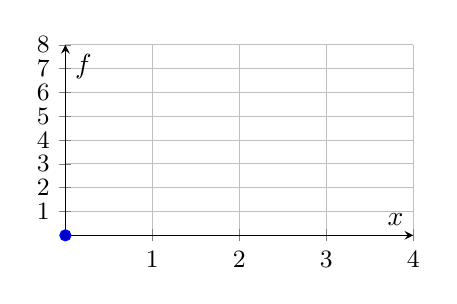
\begin{tikzpicture}
		\begin{axis}[width=6cm,height=4cm, axis background/.style={fill=white}, axis lines=middle, 
		grid = major,
		xlabel=$\small x$,
		ylabel=$\small f$, 
		xtick={0,1,2,3,4},
		ytick={0,1,2,3,4,5,6,7,8},
		tick label style={font=\small},
		xmin=0,
		xmax=4,
		ymax=8,
		legend style={font=\small,legend pos=outer north east},],
		\addplot coordinates {(0, 0)};
		\end{axis}
		
		\end{tikzpicture}
	\end{center}
\end{minipage}
  

\item Quina és la probabilitat de treure un 5 en llançar un dau? I de treure una carta d'oros d'una baralla espanyola?

\vspace{1cm}
\end{itemize}

\addanswersline[cols=1]{Avaluació inicial}{0}{[La mitjana és 5.2643, 
									 \begin{tabular}{c|c}
									 	x & f \\ \hline
									 	0 & 1  \\
									 	1 & 8  \\
									 	2 & 8 \\
									 	3 & 2 \\
									 	4 & 1 \\
									 \end{tabular} 
								 \par
								 \includegraphics[width=0.4\textwidth]{img-sol/t4-0},
								$P(5)=\frac{1}{6}$ i 	$P(Oros)=\frac{10}{40}$]}

 \end{iniaval}
\newpage

\section{Fases d'un estudi estadístic}

\begin{theorybox}
 \textbf{Definicions:}

\begin{minipage}{0.7\textwidth}
		\begin{itemize}
	\item \textbf{      Individu: }Cadascun dels objectes que s'estudien.
	
	\item \textbf{      Població: }Conjunt de tots els individus que s'estudien.
	
	\item \textbf{      Mostra:} Part de la població de la qual es prendran dades.
	\end{itemize}

\vspace{0.25cm}

	 \textbf{Variable estadística. }És l'aspecte de l'estudi i es\textbf{ classifica en:}
	\begin{itemize}
		\item \textbf{       Qualitativa:} Expressa una qualitat, com ara color, marca, etc.
		\item \textbf{        Quantitativa: }S'expressa amb un nombre.  
		\begin{itemize}
			\item \textbf{Discreta} (el nombre és enter) 
			\item \textbf{Contínua} (el  nombre pot contenir decimals).
		\end{itemize}
	\end{itemize}
\end{minipage}
\begin{minipage}{0.3\textwidth}
	\centering
	\includegraphics[width=0.9\textwidth]{img-04/mostra}
\end{minipage}




 \textbf{Fases d'un estudi estadístic:}
\begin{enumerate} 
	\item Tenir clara la pregunta i el tipus de variable estadística que es vol estudiar.  
	\item Prendre una mostra representativa.
	\item Recollir les dades (fent una enquesta, etc.) 
	\item  Fer un recompte de dades, càlculs de paràmetres estadístics i gràfics.
	\item Treure conclusions.
\end{enumerate} 
\end{theorybox}

\begin{mylist}

\exer Volem fer un estudi de la quantitat de monedes que duen a la butxaca els estudiants de la classe. Però, per no demanar a tots triam 10 companys a l'atzar i anotam en el quadern quantes monedes duu cadascun.

\begin{tasks}
	\task Quina és la població objecte de l'estudi?
	\task Quina és la mostra triada?
	\task Especifica 5 individus que pertanyin a la població i no a la mostra.
\end{tasks}
 
\answers[cols=1]{[La població són tots els alumnes de la classe, La mostra són els 10 companys triats a l'atzar, Qualssevol alumne de la classe que no hagués estat triat a l'atzar.]}
 
\exer \spen Classifica en variables qualitatives i quantitatives. Per a les quantitatives indica si són contínues o discretes.
\begin{tasks}
\task Quines fruites menges al llarg d'una setmana? \dotfill\hspace{1cm}
\task  Quantes peces de fruita menges al dia? \dotfill\hspace{1cm}
\task  Quantes monedes portes en la butxaca? \dotfill\hspace{1cm}
\task  Quina és la teva altura? \dotfill\hspace{1cm}
%\task  Quantes marques de xocolata recordes?
\task  Quines són les marques de xocolata que recordes? \dotfill\hspace{1cm}
\task  Quants germans tens? \dotfill\hspace{1cm}
\task  Quin és el teu color favorit per a un cotxe? \dotfill\hspace{1cm}
\task  Quant temps passes al dia veient la televisió? \dotfill\hspace{1cm}
\task  Quants seguidors tens en twitter? \dotfill\hspace{1cm}
\end{tasks}
\answers[cols=1]{[Qualitativa, Quantitativa Discreta, Quantitativa Discreta, Quantitativa Contínua, Qualitativa, Quantitativa Discreta, Qualitativa, Quantitativa Contínua, Quantitativa Discreta]}
 

 \exer Assenyala en quin cas és més convenient estudiar la població o una mostra:
\begin{tasks}
 \task El diàmetre dels cargols que fabrica una màquina diàriament. 
%
 \task L'altura d'un grup de sis amics. 
\end{tasks}
\answers[cols=1]{[Millor la mosta, Millor la població]}
 

 \exer Es pot llegir el següent titular en la revista que publica el teu institut: ``\textit{La nota mitjana dels alumnes de 3r ESO és }de 7,9''. Com s'ha arribat a aquesta conclusió? S'ha estudiat a tota la població? Si haguessin seleccionat per al seu càlcul tan sols a les nines, seria representatiu el seu valor?

 \answers{Segurament hauran utilitzat el programa Gestib que ho gestiona tot. En tal cas, estudien tota la població. Si l'estudi
 hagués comptat només amb les alumnes, el resultat no representaria a toda la població.}

 \exer En una sèrie de televisió tenen dubtes sobre què fer amb la protagonista, si que tingui un accident o si ha de casar-se. Volen fer una consulta; a tota la població o seleccionat una mostra representativa? Raona la resposta.

\answers{Seria molt complicat consultar a tota la població (llarg i car). Millor una mostra.}

\end{mylist}

\section{Representació de la informació}

\begin{center}
\boxed{\includegraphics[width=0.9\textwidth]{img-04/grafics}}
\end{center}

\begin{mylist}
 \exer  Reuneix a 10 companys. Compta quantes monedes de cada valor (1 cèntim, 2 cèntims, 5 cèntims, {\dots}) teniu entre tots. Representa mitjançant un gràfic adequat el nombre de monedes de cada tipus que teniu. Hi ha algun altre diagrama que et permeti veure quin tipus de monedes són més abundants en la mostra que has pres?

\answers{Solució oberta. Faríem un diagrama de sectors o de barres.}
  
 \exer En la classe d'Educació Física el professor ha mesurat el temps que tarda cada alumne a recórrer 100 metres. Els resultats estan en aquesta taula:
\begin{center}
\begin{tabular}{|p{0.4in}|p{0.4in}|p{0.4in}|p{0.4in}|p{0.4in}|p{0.4in}|p{0.4in}|p{0.4in}|} \hline 
14'92 & 13'01 & 12'22 & 16'72 & 12'06 & 10'11 & 10'58 & 18'58 \\ \hline
20'07 & 13'15 & 20'10 & 12'43 & 17'51 & 11'59 & 11'79 & 16'94 \\ \hline
16'45 & 10'94 & 16'56 & 14'87 & 17'59 & 13'74 & 19'71 & 18'63 \\ \hline
19'87 & 11'12 & 12'09 & 14'20 & 18'30 & 17'64 & &\\ \hline 
\end{tabular}
\end{center}
Agrupa aquests resultats en intervals començant en 10 segons i de longitud 1 segon. Realitza una taula de freqüències i representa adequadament aquestes dades.

\answers{
\begin{tabular}{c|c}
Interval & f \\ \hline
10 -- 11 &   3    \\ 
11 -- 12 &   3 \\ 
12 -- 13&   4 \\ 
13 -- 14&   3 \\ 
14 -- 15&   3 \\ 
15 -- 16&   0 \\ 
16 -- 17&   4 \\ 
17 -- 18&   3 \\ 
18 -- 19&   3 \\ 
19 -- 20 &  2  \\
20 -- 21 & 2 \\ \hline
 Total & 30 \\ 
\end{tabular}
\par
\includegraphics[width=0.35\textwidth]{img-sol/t4-7}
\par \ggblink{https://goo.gl/pWA3K9}
}

\end{mylist}


\section{Paràmetres estadístics}
\begin{theorybox}[Paràmetres estadístics]
	Donada una variable estadística $x_i$ amb cada valor repetit $f_i$ vegades (freqüència), es defineixen	
	
	\begin{minipage}{0.45\textwidth}
	\begin{itemize}
		\item \textbf{Nombre de dades:} $N=\sum_i f_i$
		\item \textbf{Mitjana aritmètica:} $\bar x=\dfrac{\sum_i f_i x_i}{N}$
		\item \textbf{Variància:} $Var=\dfrac{\sum_i f_i x^2_i}{N}-\bar x^2$
		\item \textbf{Desviació típica:} $\sigma=\sqrt{Var}$		
		\item \textbf{Coeficient de variació:} $CV = \dfrac{\sigma_x}{\bar x}$
	\end{itemize}
	\end{minipage}
	\hspace{0.3cm}
	\begin{minipage}{0.44\textwidth}
				\begin{itemize}
				\item \textbf{Moda:} El valor de $x$ més freqüent.
				\item \textbf{Mediana:} Valor de $x$ pel qual la {\normalfont \textit{freqüència acumulada}} assoleix el 50\%.
				\item \textbf{Rang:} La diferència entre els valors major i menor de $x$.
				 
			\end{itemize}
	\end{minipage}
	
	La mitjana és el centre de gravetat de la distribució i la desviació típica ens dóna la \textbf{dispersió}. És a dir, ens diu com d'allunyades estan les dades respecte de la mitjana. 
	Podem pensar que una dada és ``normal'' si es troba dins l'interval de $x$ $(\bar x -\sigma, \bar x + \sigma)$.
\end{theorybox}
	
	\begin{resolt}{Hem demanat pel nombre d'assignatures suspeses a un grup de 15 alumnes i aquestes han estat les respostes:\vspace{0.25cm}
			 \begin{center}
			 \begin{tabular}{cccc}
			 	1 & 0 & 3 & 2 \\
			 	0 & 6 & 2 & 5 \\
			 	3 & 2 & 4 & 3 \\
			 	4 & 1 & 3 & 	
			 \end{tabular}
		\end{center}
		\vspace{0.25cm}
		
			\begin{itemize}
				\item[a)]  Fes un recompte i dibuixa un diagrama de barres.
				
				\item[b)]  Calcula la mitjana i la desviació típica.
			\end{itemize}
		}
		
\begin{center}
\begin{minipage}{0.2\textwidth}
	\centering
	 	\begin{tabular}{|p{0.4in}|p{0.4in}|} \hline 
			$x_i$ & $f_i$ \\ \hline 
			0 & 2\\ \hline 
			1 & 2 \\ \hline 
			2 & 3 \\ \hline 
			3 & 4 \\ \hline 
			4 & 2 \\ \hline 
			5 & 1 \\ \hline 
			6 & 1  \\ \hline
		\end{tabular}
\end{minipage}	
\begin{minipage}{0.4\textwidth} 
	\centering
	\includegraphics[width=\textwidth]{img-04/histo2}
\end{minipage}
\end{center}

		\vspace{0.24cm}
		
		Per calcular els paràmetres estadístics necessitam calcular dues columnes més $f\cdot x$ i $f\cdot x^2$:
		\begin{center}
			\begin{tabular}{|p{0.7in}|p{0.8in}|p{0.8in}|p{0.8in}|} \hline 
				$x_i$ & $f_i$ & $f_i x_i$ & $f_i x_i^2$\\ \hline 
				0 & 2 & 0 & 0 \\ \hline 
				1 & 2 & 2 & 2 \\ \hline 
				2 & 3 & 6 & 12\\ \hline 
				3 & 4 & 12 & 36 \\ \hline 
				4 & 2 & 8 &  32\\ \hline
				5 & 1 & 5 &  25\\ \hline
				6 & 1 & 6 &  36\\ \hline\hline
				\rowcolor{lightgray} SUMES & 15 &  39  & 143 \\ \hline 
			\end{tabular}
		\end{center}	\vspace{0.24cm}
		
		La mitjana s'obté de $\bar x = \dfrac{39}{15}=2.6$
		
		La desviació típica  $\sigma = \sqrt{ \dfrac{143}{15}-2.6^2 }=1.67$
		
		El coeficient de variació és $CV = \dfrac{1.67}{2.6}=0.64$, aproximadament un 64\%.
		
	\end{resolt}
	\vspace{1cm}
	
	\newpage
	
	
	\begin{resolt}{En un barri s'ha trobat que les famílies residents s'han distribuït, segons el número de membres, de la forma següent:\vspace{0.25cm}
			
			\begin{tabular}{|p{0.7in}|p{0.8in}|} \hline 
				\textbf{\textit{membres}} & \textbf{\textit{nº famílies}} \\ \hline 
				0-2 & 110 \\ \hline 
				2-4 & 200 \\ \hline 
				4-6 & 90 \\ \hline 
				6-8 & 75 \\ \hline 
				8-10 & 25 \\ \hline 
			\end{tabular}
			\vspace{0.25cm}
			
			\begin{itemize}
				\item[a)]  Representa un histograma.
				
				\item[b)]  Calcula la mitjana i la desviació típica.
			\end{itemize}
		}
		
		\begin{wrapfigure}{R}{0.3\textwidth} 
			\vspace{-0.75cm}
			\begin{center}
				\includegraphics[width=0.26\textwidth]{img-04/histo1}
			\end{center}
			\vspace{-0.5cm}
		\end{wrapfigure}
		
		a)
		\vspace{0.24cm}
		
		Es tracta d'una variable discreta (número de membres) que s'ha agrupat en intervals. El número de famílies és la freqüència. Aleshores, el gràfic més adequat és fer un histograma.
		\vspace{0.24cm}
		
		Per calcular els paràmetres estadístics necessitam calcular \textbf{la marca de classe} que és el punt mitjà de cada interval.
		\begin{center}
			\begin{tabular}{|p{0.7in}|p{0.8in}|p{0.8in}|p{0.8in}|} \hline 
				$x_i: marca$ & $f_i$ & $f_i x_i$ & $f_i x_i^2$\\ \hline 
				1 & 110 & 110 & 110 \\ \hline 
				3 & 200 & 600 & 1800 \\ \hline 
				5 & 90 & 450 & 2250\\ \hline 
				7 & 75 & 525 & 3675 \\ \hline 
				9 & 25 & 225 & 2025 \\ \hline\hline
				\rowcolor{lightgray} SUMES & 500 & 1910 & 9860\\ \hline 
			\end{tabular}
		\end{center}	\vspace{0.24cm}
		
		b)
		\vspace{0.24cm}
		
		
		La mitjana s'obté de $\bar x = \dfrac{1910}{500}=3.82$
		
		La desviació típica  $\sigma = \sqrt{ \dfrac{9860}{500}-3.82^2 }=2.26$
		
		El coeficient de variació és $CV = \dfrac{2.26}{3.82}=0.57$, aproximadament un 60\%.
		
	\end{resolt}
	\vspace{1cm}

\begin{mylist}
	
\exer[1]  En una excursió de muntanya participen 25 persones amb les següents edats: 
\begin{center}
	\begin{tabular}{|p{0.27in}|p{0.27in}|p{0.27in}|p{0.27in}|p{0.27in}|p{0.27in}|p{0.27in}|p{0.27in}|p{0.27in}|p{0.27in}|p{0.27in}|p{0.27in}|p{0.27in}|} \hline
		8 & 10 & 10 & 11& 12& 36& 37& 37& 38& 40& 42& 43& 43 \\ \hline  
		44 & 45 & 47 & 48& 50& 52& 53& 55& 58& 61& 63& 67&  \\ \hline 
\end{tabular}
\end{center}
\begin{tasks}
\task Fes una taula de freqüències classificant les edats en 6 intervals que comencen en 7,5 i acaben en 67,5. Troba, a partir de la taula, els paràmetres $\bar{x}$, $\sigmaup$  i CV.
\task Calcula $\bar{x}$, $\sigmaup$  i CV  introduint els 25 dades en la calculadora, és a dir, sense agrupar-los en intervals.
\task Prescindint dels 5 nins, obtenim un col·lectiu de 20 persones. Calcula de nou els seus paràmetres $\bar{x}$, $\sigmaup$ i CV,  i compara amb els obtinguts en el grup inicial.
\end{tasks}

\answers[cols=1]{[$\bar x=40.5$; $\sigma=16.5$; $CV=0.407$,  $\bar x=40.4$; $\sigma=17.11$; $CV=0.424$, $\bar x=46.5$; $\sigma=9.74$; $CV=0.21$ \par \ggblink{https://goo.gl/JfqFSu}]}

\end{mylist}


\newpage

 \section{Problemes d'estadística}

\begin{mylist}
	
 \exer[1] S'han recollit les dades sobre el nombre de fills que tenen 20 matrimonis. Com és la variable utilitzada? Escriu una taula de freqüències de les dades recollides i representa les dades en un diagrama de sectors:  
\begin{center}
3, \quad 1,\quad 1, \quad2,\quad0, \quad2, \quad3, \quad1,\quad 1,\quad 1,\quad 1, \quad0, \quad3, \quad2, \quad1,\quad 2,\quad 1,\quad 2,\quad 2,\quad 3
\end{center}
 Amb aquestes dades calcula la moda, la mitjana, la variància i la desviació típica. 
  
\answers{$M_o =1$; $\bar x=1.6$; $Var=0.84$; $\sigma=0.92$\par
\ggblink{https://goo.gl/nKce19}}

\vso

 \exer[1] Es demana a un grup de persones pel nombre de televisors que hi ha en casa seva i els resultats han estat: 

\begin{longtable}{|p{1.2in}|p{0.2in}|p{0.2in}|p{0.2in}|p{0.2in}|p{0.2in}|p{0.2in}|} \hline 
Nombre de \par televisors & 0 & 1 & 2 & 3 & 4 & 5 \\ \hline 
Nombre de llars & 2 & 27 & 15 & 4 & 2 & 1 \\ \hline 
\end{longtable}

Quin tipus de variable és? Representa les dades en la representació que et sembli més adequada. Calcula la mitjana i la desviació típica.

\answers{Variable quantitativa discreta;\par $\bar x=1.6078$; $\sigma=0.9717$\par \ggblink{https://goo.gl/9tu6n7}}

\vso

\exer[1] En un centre escolar s'ha recollit informació sobre el nombre d'ordinadors a les cases de 100 famílies i s'han obtingut els següents resultats: 

\begin{longtable}{|p{1.3in}|p{0.3in}|p{0.3in}|p{0.3in}|p{0.3in}|p{0.3in}|} \hline 
Nombre \par d'ordinadors & 0 & 1 & 2 & 3 & 4 \\ \hline 
Nombre de \par famílies: & 24 & 60 & 14 & 1 & 1 \\ \hline 
\end{longtable}

Representa les dades en un diagrama de barres i calcula la mitjana, la mediana i la moda.
\answers{$\bar x=0.95$;  $M_o=1$; $M_e$ = 1; $Q_1 = 1$; $Q_3= 1$
	\par
	\ggblink{https://goo.gl/nFytiW}
}
 
\exer Amb les dades del problema anterior calcula el rang, la desviació mitjana, la variància i la desviació típica. 


\answers{Rang = 4. Desviació mitjana = 0,456. Variància = 0,299. Desviació típica = 0,5473; \par \ggblink{https://goo.gl/nFytiW}}

\vso

 \exer Es demana a un grup de persones pel nombre de vegades que han visitat al dentista en l'últim any. Les respostes obtingudes es recullen en la següent taula: 

\begin{longtable}{|p{1.5in}|p{0.5in}|p{0.5in}|p{0.5in}|p{0.5in}|p{0.5in}|} \hline 
Nombre de visites: & 1 & 2 & 3 & 4 & 5 \\ \hline 
Nombre de persones: & 13 & 18 & 7 & 5 & 7 \\ \hline 
\end{longtable}

\begin{tasks}
	\task Representa les dades en un diagrama de sectors i calcula la mitjana, la mediana i la moda.
	\task Calcula el rang, la desviació mitjana, la variància i la desviació típica.	
\end{tasks}

\answers{[Mitjana = 2.5; Mediana = 2; Moda = 2; Var=1.81; $\sigma=1.345$;  CV=0.538, \includegraphics[width=0.35\textwidth]{img-sol/t4-13}\par \ggblink{https://goo.gl/RtMKif}]}
 
\newpage

\exer  En un control de velocitat en carretera s'obtingueren les dades següents

\begin{longtable}{|p{1.3in}|p{0.5in}|p{0.5in}|p{0.5in}|p{0.5in}|p{0.7in}|p{0.7in}|} \hline 
Velocitat (km/h): & 60--70 & 70--80 & 80--90 & 90--100 & 100-110 & 110-120 \\ \hline 
Nombre de cotxes: & 5 & 15 & 27 & 38 & 23 & 17 \\ \hline 
\end{longtable}

\begin{tasks}
	\task Calcula la mitjana i la desviació típica de la velocitat dels cotxes. {\textit Ajuda: } La marca de classe de l'interval 60--70 és 65.
	\task Quin percentatge circula a més de 90 km/h?
\end{tasks}
 
 \answers{[$\bar x=93.8$; $\sigma=13.3$; $CV=0.142$,  62.4 \% \par \ggblink{https://goo.gl/t62BLv}]}

\vso
\exer  La següent taula expressa les alçades, en metres, de 1000 soldats: 

\begin{longtable}{|p{0.9in}|p{0.5in}|p{0.5in}|p{0.5in}|p{0.5in}|p{0.5in}|p{0.5in}|} \hline 
Talla & 1,50 -- 1,56 & 1,56 -- 1,62 & 1,62 -- 1,68 & 1,68 - 1,74 & 1,74 - 1,80 & 1,80-1,86 \\ \hline 
Nº de soldats & 10 & 140 & 210 & 340 & 210 & 90 \\ \hline 
\end{longtable}

\begin{tasks}
	\task Representa les dades en un histograma.
	\task Calcula la mitjana i la desviació típica. 
	\task Determina l'interval on es troba la mediana.
\end{tasks}
\answers{[\includegraphics[width=0.35\textwidth]{img-sol/t4-15},
		Mitjana = 1.7049. Desviació típica =0.07132,
Mediana. Per a calcular l'interval on es troba miram, en
 la taula de les freqüències acumulades, estan els 500 soldats. És l'interval 1,68 – 1,74.\par 
 \ggblink{https://goo.gl/QVSssH}
 ]}
 

 \begin{comment}
 \exer En les eleccions de 2014 al Parlament Europeu es van obtenir els següents escons per grup parlamentari (DM: demòcrata -- cristians; S: socialistes; L: Liberals; V: verds; C: conservadors; I: esquerra unitària; LD: Llibertat i democràcia; NI: No inscrits; Uns altres). 

\begin{longtable}{|p{0.7in}|p{0.3in}|p{0.3in}|p{0.3in}|p{0.3in}|p{0.3in}|p{0.3in}|p{0.3in}|p{0.3in}|p{0.4in}|p{0.4in}|} \hline 
Partits & DM & S & L & V & C & I & LD & NI & Uns altres & Total \\ \hline 
Escons & 213 & 190 & 64 & 52 & 46 & 42 & 38 & 41 & 65 & 751 \\ \hline 
\end{longtable}

Quina representació de les dades et sembla més adequada? Pots calcular la mitjana o el rang? Quin tipus de variables és la de la taula?


\exer  En les eleccions de 2014 al Parlament Europeu es van obtenir els següents escons per algun dels estats membre: 

\begin{longtable}{|p{0.5in}|p{0.5in}|p{0.5in}|p{0.5in}|p{0.5in}|p{0.5in}|p{0.5in}|p{0.5in}|p{0.5in}|p{0.5in}|p{0.5in}|} \hline 
Estat & Alemanya & Espanya & França & Itàlia & Polònia & Regne Unit & Portugal & Grècia & Uns altres & Total \\ \hline 
Escons & 96 & 54 & 74 & 73 & 51 & 73 & 21 & 21 &  & 751 \\ \hline 
\end{longtable}

Quina representació de les dades et sembla més adequada? Pots calcular la mitjana o el rang? Quin tipus de variables és la de la taula? Determina el nombre d'escons dels altres països membres de la Unió Europea.
\end{comment}

\vso
 \exer En les eleccions de 2004, 2009, 2014 al Parlament Europeu es van obtenir els següents percentatges de vots per alguns dels estats membres: 

\begin{longtable}{|p{0.4in}|p{0.6in}|p{0.5in}|p{0.4in}|p{0.4in}|p{0.4in}|p{0.5in}|p{0.4in}|p{0.5in}|p{0.5in}|} \hline 
Estat & Alemanya & Espanya & França & Itàlia & Regne Unit & Portugal & Grècia & Bèlgica & \% total \\ \hline 
2004 & 43 & 45'14 & 42'76 & 71'72 & 38'52 & 38'6 & 63'22 & 90'81 & 45'47 \\ \hline 
2009 & 43'27 & 44'87 & 40'63 & 65'05 & 34'7 & 36'77 & 52'61 & 90'39 & 43 \\ \hline 
2014 & 47'6 & 45'9 & 43'5 & 60 & 36 & 34'5 & 58'2 & 90 & 43'09 \\ \hline 
\end{longtable}

Quina representació de les dades et sembla més adequada? Pots calcular la mitjana o el rang? Quin tipus de variables és la de la taula? Ordena als països de major a menys percentatge de votants en les eleccions de 2014.
\vso
\answers{Es pot representar mitjançant un diagrama de barres amb colors diferents per a cada any. La variable és
	quantitativa contínua i es poden calcular paràmetres estadístics. L'ordre dels països és Bèlgica$>$
	Itàlia $>$ Grècia $>$ Espanya $>$ Alemanya $>$ França $>$ Portugal $>$ Regne Unit.\par  
\ggblink{https://goo.gl/Z6UoWb}}

\exer  En les eleccions de 2014 al Parlament Europeu els resultats d'Espanya han estat: 

\begin{longtable}{|p{0.9in}|p{0.9in}|p{0.9in}|p{0.9in}|p{0.9in}|} \hline 
Cens & Total de votants & Abstenció & Vots nuls & Vots en blanc \\ \hline 
35.379.097 & 15.620.815 & 19.058.282 & 290.189 & 409.811 \\ \hline 
\end{longtable}

Representa en un diagrama de sectors aquestes dades. Fes una taula de percentatges: el cens és el 100 \%. Determina els altres percentatges. Consideres que ha guanyat l'abstenció?

\answers{ 
	\includegraphics[width=0.4\textwidth]{img-sol/t4-17}
	 \par
	Cens=100 \%;\par
	Total de votants=
	44,152 \%; \par
	Abstenció=
	53,87 \%; \par
	Vots nuls=
	0,82022727 \%; \par
	Vots en blanc=
	1,1583\%; \par
	Ha guanyat l'abstenció, amb més de la meitat del cens.\par 
\ggblink{https://goo.gl/JjcnL4}}
   
\begin{comment}
 \exer En les eleccions de 2014 al Parlament Europeu els resultats d'Espanya han estat: 

\begin{longtable}{|p{0.7in}|p{0.7in}|p{0.7in}|p{0.7in}|p{0.7in}|p{0.7in}|p{0.7in}|} \hline 
\textbf{PP} & \textbf{PSOE} & \textbf{Esquerra plural} & \textbf{Podemos} & \textbf{UPyD} & \textbf{Uns altres} & \textbf{Total de votants} \\ \hline 
4.074.363 & 8.001.754 & 1.562.567 & 1.245.948 & 1.015.994 &  & 15.920.815 \\ \hline 
\end{longtable}

Determina el nombre de vots dels altres partits. Representa en un diagrama de barres aquestes dades. Fes una taula de percentatges per a cada partit. Has de distribuir 54 escons, com els distribuiries per partits?
\end{comment}
\end{mylist} 

\newpage

\section{Introducció al càlcul de probabilitats}
\begin{theorybox}
 \video[ytid=R9ZSI6Rq9Yw]{155}{Introducció a la probabilitat}

                 - Experiències deterministes i \textbf{aleatòries} (hi intervé l'atzar).                                     
                 
                 \textbf{- Espai Mostral E}: Conjunt de tots els possibles resultats d'un experiment aleatori.

 La \textbf{probabilitat} és una mesura de quant freqüent és un \textbf{succés}. Es quantifica amb un nombre que com a mínim val 0 (succés impossible) i com a màxim 1 (succés segur).

 La probabilitat (experimental) és el valor de la \textbf{freqüència relativa} (freqüència / nombre de repeticions) quan repetim l'experiment moltes vegades.

 Si $S'$ i $S$ són \textbf{successos contraris}, es compleix que $P(S')=1-P(S)$.
\end{theorybox}
                                               
\begin{mylist}
\exer \mental Per a cadascun d'aquests experiments indica si és determinista o aleatori.
\begin{tasks} 
	\task  Treim una carta a l'atzar d'una baralla espanyola i mirem el pal.
	\task  Treim una bola d'una bossa que només conté boles vermelles i miram el color.
	\task  Mesurem la quantitat de gasoil que cap en dipòsit el nostre cotxe.
	\task  Cronometram el temps que tardam d'anar de casa al col·legi en diferents dies.
	\task  Llancem dos daus i mirem si ha sortit igual puntuació en els dos.
\end{tasks}
\answers[cols=1]{[Aleatori, Determinista, Determinista, Aleatori, Aleatori]}

\exer  Una baralla francesa té 52 cartes, distribuïdes en 13 cartes de piques, 13 de cors, 13 de trèvols i 13 de diamants. Les piques i els trèvols són cartes negres mentre que els cors i els diamants són cartes vermelles. Es barreja la baralla, es talla i es fa el següent experiment: agafar les dues cartes que han quedat a dalt del tot i observar de quin color són. Descriu l'espai mostral. 
\answers{E=$\{VV, VN, NV, NN \}$}
  
\vspace{-2cm}
\exer \simbolsearch \begin{minipage}[t]{0.7\textwidth} \textit{\bf Experiment llançament de monedes}.
	 Agafa una moneda d'un euro per exemple. Primer de tot, decideix quina banda és cara (C) i quina creu (X). Ara llança la moneda 10 vegades i compta quantes cares han sortit.  Tot seguit, el professor anirà demanant a cada grup quins han estat els resultats i els apuntarem en aquesta taula
	\end{minipage}
\begin{minipage}{0.3\textwidth}
	\vspace{2cm}
	\centering
	\includegraphics[width=0.7\textwidth]{img-04/monedes}
\end{minipage}
	

\begin{longtable}{|p{0.7in}|p{0.2in}|p{0.2in}|p{0.2in}|p{0.2in}|p{0.2in}|p{0.2in}|p{0.2in}|p{0.2in}|p{0.2in}|p{0.2in}|p{0.2in}|p{0.2in}|p{0.2in}|p{0.2in}|} \hline 
N. Tirades & 10 & 20 & 30 & 40 & 50 & 60 & 70 & 80 & 90 & 100 & 110 & 120 & 130 & 140 \\ \hline 
N. Cares &  &  &  &  &  &  &  &  &  &  &  &  &  &  \\ \hline 
Freq.\newline relativa &  &  &  &  &  &  &  &  &  &  &  &  &  &  \\ \hline 
\end{longtable}
  En la segona fila de la taula, anirem acumulant el nombre de cares que han anat sortint a cada grup. En la tercera fila, calcularem la freqüència relativa, és a dir, el nombre de cares dividit pel nombre de tirades. Amb aquests resultats contesta:
\begin{tasks} 
\task Quina és la probabilitat experimental d'obtenir cara? I d'obtenir creu?
\task Són equiprobables els successos treure cara i treure creu? Per què?
\end{tasks}

\answers{\href{https://piworld.es/\#!/home/activity/71/0}{Simulació}:\par
	\includegraphics[width=0.4\textwidth]{img-sol/t4-sim-monedes} \par
\begin{tasks} \task Pel nombre més alt de tirades, cerca la freqüència relativa. Aquesta és la millor aproximació a la probabilitat d'obtenir cara. La probabilitat de treure creu és $P(X)=1-P(C)$ \task Sí. Són equiprobables. Perquè la moneda és simètrica i no està trucada.\end{tasks}}

\pagebreak
 
 \mbox{}
\vspace*{-2.5cm}
\exer \simbolsearch \begin{minipage}[t]{0.7\textwidth}  \textit{\bf Experiment llançament de xinxetes}. Agafa una xinxeta i fixeu-vos que pot caure de dues formes: punxa per amunt o de costat. Ara llança la xinxeta 10 vegades i compta quantes han sortit punxa per amunt. Tot seguit, el professor anirà demanant a cada grup quins han estat els resultats i els apuntarem en aquesta taula
	\end{minipage}
\begin{minipage}{0.3\textwidth}
\vspace{2cm}
\centering
\includegraphics[width=0.8\textwidth]{img-04/xinxetes}
\end{minipage}

\begin{longtable}{|p{0.7in}|p{0.2in}|p{0.2in}|p{0.2in}|p{0.2in}|p{0.2in}|p{0.2in}|p{0.2in}|p{0.2in}|p{0.2in}|p{0.2in}|p{0.2in}|p{0.2in}|p{0.2in}|p{0.2in}|} \hline 
	N. Tirades & 10 & 20 & 30 & 40 & 50 & 60 & 70 & 80 & 90 & 100 & 110 & 120 & 130 & 140 \\ \hline 
	N. Amunt &  &  &  &  &  &  &  &  &  &  &  &  &  &  \\ \hline 
	Freq.\newline relativa &  &  &  &  &  &  &  &  &  &  &  &  &  &  \\ \hline 
\end{longtable}

En la segona fila de la taula, anirem acumulant el nombre de pics que cau la punxa per amunt. En la tercera fila, calcularem la freqüència relativa, és a dir, el nombre de punxes per amunt dividit pel nombre de tirades. Amb aquests resultats contesta:

\begin{tasks}
\task Quina és la probabilitat experimental de caure punxa per amunt? I  de caure de costat?
\task Són equiprobables els dos successos? Per què?
\end{tasks}

\answers[cols=1]{[Pel nombre més alt de tirades, cerca la freqüència relativa. Aquesta és la millor aproximació a la probabilitat de caure per amunt. La probabilitat de caure de costat és $P(costat)=1-P(amunt)$, No són equiprobables. Perquè la xinxeta pesa més d'una banda que de l'altre. Les dues bandes no són  simètriques.]}
\vso
 

\exer \mental En una bossa tenim 10 boles vermelles numerades de l'1 al 10. Es fan els dos experiments següents: 

 \quad EXPERIMENT A: Es treu una bola de la bossa i es mira el seu color.

 \quad EXPERIMENT B: Es treu una bola de la bossa i es mira el seu nombre.

 Quin d'aquests experiments no és un experiment aleatori? Per què?

 Pel cas que sigui un experiment aleatori, descriu el seu espai mostral.
\answers{L'experiment A és determinista perquè segur que surt bola vermella. L'experiment B és aleatori perquè no sabem el nombre que sortirà abans de fer l'experiment. L'espai mostral és E=\{1, 2, 3, 4, 5, 6, 7, 8, 9, 10\}}
\end{mylist}


  
\section{Probabilitats simples (Regla de Laplace)}

\begin{theorybox}
\video[ytid=hpag1\_CTp4k]{156}{Probabilitat: Regla de Laplace}  

                 Si tots els possibles resultats d'un experiment aleatori tenen la mateixa probabilitat (són \textbf{equiprobables}), podem aplicar la \textbf{regla de Laplace}:
\[P\left(S\right)=\frac{Nombre\ de\ casos\ favorables\ a\ S}{Nombre\ de\ casos\ totals}\] 
    \vspace{0.5cm}
\end{theorybox}
 
\pagebreak
 \begin{mylist}

\exer \spen  Troba la probabilitat d'obtenir un 2 i la probabilitat d'obtenir un 5, en llançar un dau correcte en cada un d'aquests casos:

\begin{longtable}{p{1.5in}p{1.2in}p{1.2in}} 
	\centering 
a) Dau cúbic (6 cares)\newline \includegraphics*[bb=0 0 0.66in 0.70in, width=0.66in, height=0.70in, keepaspectratio=false]{img-04/image3.png} & b) Dau tetraèdric (4 cares)\newline \includegraphics*[bb=0 0 0.73in 0.74in, width=0.73in, height=0.74in, keepaspectratio=false]{img-04/image4.png} & c) Dau octaèdric (8 cares)\newline \includegraphics*[bb=0 0 1.13in 0.89in, width=0.78in, height=0.76in, keepaspectratio=false, trim=0.31in 0.04in 0.04in 0.09in]{img-04/image5.png} \\ [0.5cm] \quad P(2) = ........ & \quad P(2) =......... & \quad P(2)=.......... \\  [0.2cm] \quad P(5) = ........ & \quad P(5) =......... & \quad P(5).......... \\
\end{longtable}

\answers{[$P(2)=\frac{1}{6}$; $P(5)=\frac{1}{6}$,  $P(2)=\frac{1}{4}$; $P(5)=0$,  $P(2)=\frac{1}{8}$; $P(5)=\frac{1}{8}$]}


  \exer \spen En una bossa hi ha 6 boles vermelles, 4 de blaves, 7 de verdes, 2 de grogues i una de negra. En treim una a l'atzar, calcula la probabilitat de que
\begin{tasks}(2)
	\task  Sigui blava.    
	\task  No sigui negra.
	\task  Sigui vermella o verda.   
	\task  No sigui groga ni negra.
\end{tasks}
\answers{[$\frac{4}{20}$, $\frac{19}{20}$, $\frac{13}{20}$, $\frac{17}{20}$]}
 

\exer  Raona de quina de les bosses següents és més probable treure una bola negra:
\begin{center}
 \includegraphics*[  width=2.91in ]{img-04/image6.png}
\end{center}
\answers{De la bossa I. Perquè P(I)=$\frac{2}{3}=0.666...$, P(II)=$\frac{4}{7}=0.571$ i P(III)=$\frac{3}{5}=0.6$}

\exer \spen Llançam un dau regular. Calcula les probabilitats que el resultat sigui:
\begin{tasks}(2)
	\task    Múltiple de  3   
	\task  Múltiple de 2
	\task    Major que 1    
	\task  Menor que 5
	\task    Menor que 1   
	\task   Potència de 2
\end{tasks}
 \answers{[$\frac{2}{6}$, $\frac{3}{6}$, $\frac{5}{6}$, $\frac{4}{6}$, 0, $\frac{3}{6}$]}

\exer \spen  Extreim una carta d'una baralla espanyola de 40 naips. Calcula la probabilitat que:
\begin{tasks} 
\task  La carta sigui de BASTOS
\task  La carta NO sigui ni AS ni FIGURA
\task  La carta sigui menor que 6
\task  La carta sigui d'OROS o FIGURA
\end{tasks}
\answers{[$\frac{10}{40}$, $\frac{24}{40}$, $\frac{20}{40}$, $\frac{19}{40}$]}
 
 \exer  Extreim una carta d'una baralla espanyola de 40 naips. Troba la probabilitat que:
 \begin{tasks}(2)
 	\task  Sigui un CINC    
 	\task  No sigui un CAVALL
 	\task     Sigui d'OROS o de COPES   
 	\task  No sigui d'ESPASES
 \end{tasks}
 \answers{[$\frac{4}{40}$, $\frac{36}{40}$, $\frac{20}{40}$, $\frac{30}{40}$]}
\newpage

 \exer[1] En un llibre de 120 pàgines, hem comptat el nombre d'errades en cadascuna de les pàgines. Els resultats han estat: 

\begin{longtable}{|p{2.3in}|p{1.4in}|} \hline 
\textbf{Nº d'errades} & \textbf{Nº de pàgines} \\ \hline 
0 & 58 \\ \hline 
1 & 42 \\ \hline 
2 & 16 \\ \hline 
3 & 3 \\ \hline 
4 & 1 \\ \hline 
\end{longtable}

Si triam una pàgina a l'atzar:
\begin{tasks} 
	\task  Quina és la probabilitat que no tingui cap errada?
	\task  Quina és la probabilitat que tingui exactament dues errades?
	\task  I la probabilitat que tingui alguna errada? I que tingui més de tres?
\end{tasks}
\answers[cols=3]{[$\dfrac{58}{120}$, $\dfrac{16}{120}$, $\dfrac{62}{120}$  i $\dfrac{1}{120}$ ]}
 

  

\exer  D'aquesta urna extreim una bola i n'observam el nombre i el color. Calcula les probabilitats dels successos següents:
\begin{center}
	\includegraphics[width=5cm]{img-04/image11}
\end{center}
\begin{tasks} 
	\task  Obtenir una bola blanca amb un nombre parell
	\task  Obtenir bola negra amb nombre parell
	\task  Obtenir bola grisa o negre
	\task  Obtenir una bola amb nombre més gran que 7
\end{tasks}

\answers{[$\frac{2}{10}$, $\frac{1}{10}$, $\frac{7}{10}$, $\frac{3}{10}$]} 

\exer  D'una bossa amb 7 boles vermelles, 5 de verdes, 3 de grogues, 11 de negres i 3 de blaves, en treim una a l'atzar. Quina és la probabilitat que 
\begin{tasks} 
	\task    Sigui vermella?    
	\task  No sigui negra?
\end{tasks}
\answers{[$\frac{7}{29}\approx 0.24$, $\frac{18}{29}\approx 0.62$]}

\end{mylist}


\section{Probabilitat composta}

\begin{theorybox}
 \videonw[ytid=zLGB4hZyNeI]{157}{Probabilitat successos composts independents}

                      Si A i B són successos independents, es compleix que \textbf{P(A i B) = P(A)·P(B)                           }
                      
                      \normalfont{\textit{Per exemple}}: Treure dues cartes\textbf{ amb reemplaçament} (les tornam a ficar).

\videonw[ytid=3v1p6nXos\_s]{159}{Probabilitat successos composts dependents} 

                     \normalfont{\textit{Per exemple}}: Treure dues cartes \textbf{sense reemplaçament} (no les tornam a ficar). Utilitzam la tècnica de    \textbf{ diagrames d'arbre}.
\end{theorybox}

\subsection{Successos independents}

\begin{resolt}[E]{
	
Llançam un dau i treim una carta d'una baralla espanyola de 40 cartes. Quina és la probabilitat d'obtenir múltiple de 3 al dau i rei a la carta?
	
}
	\textbf{Compost independent}

	\[P(\text{\boxed{3,6} i \boxed{rei}})= P(\text{\boxed{3,6}}) \cdot P(\text{\boxed{rei}}) = \frac{2}{6}\cdot \frac{4}{40}=\frac{1}{30} \]
	
\end{resolt}

\begin{mylist}
	

\exer Llançam un dau i una moneda. Calcula les probabilitats:
\begin{tasks}(2)
	\task  Treure un 6 i cara     
	\task  Treure parell i creu.
\end{tasks}
\answers{[$\frac{1}{6}\cdot \frac{1}{2}=\frac{1}{12}$, $\frac{3}{6}\cdot \frac{1}{2}=\frac{1}{4}$]}


\exer  Es considera l'experiment aleatori de tirar un dau dues vegades. Calcula les probabilitats següents:  
\begin{tasks}(2)
	\task  Treure algun 1.     
	\task  La suma dels dígits és 8. 
	\task  No treure cap 2.    
	\task  Treure algun 1 o bé no treure cap 2.
\end{tasks}
 \answers{Si $A$=\{1,2,3,4,5,6\}, cal calcular el producte cartesià $A\times A$.\par
\begin{tasks}(2) \task $\frac{11}{36}$ \task  $\frac{5}{36}$ \task  $\frac{25}{36}$ \task  $\frac{31}{36}$\end{tasks}}
  
\exer[1]  Es considera l'experiment aleatori de tirar una moneda tres vegades. Calcula les probabilitats següents:  
\begin{tasks}(2) 
	\task  Treure cara en la primera tirada.   
	\task  Treure cara en la segona tirada.
	\task  Treure cara en la tercera tirada.  
	\task  Treure alguna cara. 
	\task  No treure cap cara.     
	\task  Treure tres cares. 
\end{tasks}
\answers[cols=3]{[$\frac{1}{2}$, $\frac{1}{2}$, $\frac{1}{2}$, $1-\dfrac{1}{8}=\dfrac{7}{8}$, $\frac{1}{8}$, $\frac{1}{8}$]}

 \exer[1]  Es considera l'experiment aleatori treure dues cartes de la baralla espanyola amb reemplaçament. Calcula la probabilitat de:  
 \begin{tasks}(2)
 	\task  Treure algun rei.        
 	\task  Obtenir almenys un basto. 
 	\task  No obtenir cap basto.       
 	\task  No obtenir el rei de bastos. 
 	\task  Treure figura: sota, cavall, rei o as.     
 	\task  No treure cap figura.
 \end{tasks}
 \answers[cols=3]{[0.19, 0.44, 0.56, 0.95, 0.65, 0.35]}

\newpage

\exer  En llançar quatre monedes a l'aire,  
\begin{tasks}
	\task  Quina és la probabilitat que les quatre siguin cares?
	\task  Quina és la probabilitat d'obtenir com a màxim tres cares? 
	\task  Quina és la probabilitat de tenir exactament 3 cares?
\end{tasks}
\answers[cols=1]{[$\left(\frac{1}{2}\right)^4= \frac{1}{16}$, $1-P(CCCC)=1-\frac{1}{16}=\frac{15}{16}$, $4 P(XCCC)=4\left(\frac{1}{2}\right)^4=\frac{1}{4}$]}
  

 \exer[1] \label{list:boles} En una urna hi ha 6 boles blanques i 14 boles negres. Es treuen dues boles amb reemplaçament. Determina la probabilitat que: 
\begin{tasks}(2)
	\task  Les dues siguin negres.  
	\task  Hi hagi almenys una negra.  
	\task  Cap sigui negra.
\end{tasks}
\answers[cols=3]{[$\dfrac{49}{100}$, $\dfrac{91}{100}$, $\dfrac{9}{100}$]}

\subsection{Successos dependents. Diagrames d'arbre}

\begin{resolt}[E]{
	 Dos tiradors al plat tenen unes marques ja conegudes. El primer encerta amb una probabilitat de 0,7 i el segon de 0,4. Es llança un plat i tots dos disparen. Expressa mitjançant un diagrama d'arbre i les diferents possibilitats: 
	 \vspace{0.5cm}
	 
	 \begin{tasks}
	 	\task  Calcula la probabilitat que cap encerti.
	 	\task  Calcula la probabilitat que els dos encertin.
	 	\task  Quina probabilitat hi ha que un dels tiradors doni en el plat?
	 \end{tasks}
}
	Per resoldre aquest problema, utilitzam la tècnica del diagrama d'arbre 
	
	Recorda: Les probabilitats d'un camí de l'arbre es multipliquen. Diferents camins es sumen:
	
	\begin{center}
	\includegraphics[width=4.5cm]{img-04/arbre}
	\end{center}
	
	a) $P(No-No)=0,3 \cdot 0,6 = 0,18$
	
	b) $P(Si-Si)=0,7 \cdot 0,4 = 0,28$
	
	c) $P(Un)= P(No-Si)+P(Si-No) = 0,3 \cdot 0,4 + 0,7\cdot 0,6 = 0,54$
	
\end{resolt}
 
\exer[1]  En una urna hi ha 6 boles blanques i 14 boles negres. Es treuen dues boles sense reemplaçament. Determina la probabilitat que: 
\begin{tasks}
	\task  Les dues siguin negres. 
	\task  Hi hagi almenys una negra.
	\task  Cap sigui negra.
	\task  Compara els resultats amb els de l'activitat \ref{list:boles}.
\end{tasks}
\answers[cols=3]{[$\dfrac{91}{190}$, $\dfrac{35}{38}$, $\dfrac{3}{38}$]}

 \exer Amb una baralla espanyola es fa l'experiment de treure tres cartes amb reemplaçament.
	   Quina és la probabilitat de treure tres reis? 
	   I si l'experiment es fa sense reemplaçament, quin és ara la probabilitat de tenir 3 reis? 
 
 \answers[cols=1]{[Amb reemplaçament $P(RRR)=\frac{4}{40}\cdot \frac{4}{40} \cdot \frac{4}{40} =\frac{1}{1000}=0.001$,
 	Sense reemplaçament $P(RRR)=\frac{4}{40}\cdot \frac{3}{39} \cdot \frac{2}{38} =\frac{1}{2470}=0.0004$]}
 
 \newpage

\exer  Es llança una moneda fins que aparegui cara dues vegades seguides. 

\begin{tasks}
	\task  Calcula la probabilitat que l'experiment acabi en el segon llançament.
	\task  Calcula la probabilitat que acabi en el tercer llançament.
\end{tasks}
\answers[cols=1]{[$P(CC)=\frac{1}{4}$, $P(XCC)=\frac{1}{8}$]}
 

\exer[1]  En el llançament de naus espacials s'han instal·lat tres dispositius de seguretat A, B i C. Si falla A se posa automàticament en marxa el dispositiu B, i si falla aquest, s'engega C. Se sap que la probabilitat que falli A és 0,1, la probabilitat que B funcioni és 0,98 i la probabilitat que falli C és 0,05. Calcula la probabilitat que tot funcioni bé. 
\answers{$P=0.9999$}
  

 \exer Es fa un estudi sobre els incendis forestals d'una zona i es comprova que el 40 \% 
 són intencionats, el 50 \% es deuen a negligències i el 10 \% a causes naturals. 
 S'han produït dos incendis, quina és la probabilitat que

 \begin{minipage}{0.8\textwidth}
	\begin{tasks}
		\task  els dos incendis es deguin a causes naturals.
		\task  almenys un hagi estat intencionat?
		\task  cap incendi sigui per negligències.
	\end{tasks}
\end{minipage}
\begin{minipage}{0.15\textwidth}
	\centering
	\includegraphics[width=0.7\textwidth]{img-04/incendi}
\end{minipage}

\answers{\includegraphics[width=0.35\textwidth]{img-sol/t4-42} \par
\begin{tasks} \task $P=0,1\cdot 0,1 = 0,01$ 
			  \task $P=1-P(cap intencionat)= 1 - [0,5\cdot (0,5+0,1) + 0,1\cdot (0,5+0,1)]=0,64$, $P=0,25$ \end{tasks}}

\exer  Es llança dues vegades un dau equilibrat amb sis cares. Trobar la probabilitat que la suma dels valors que apareixen en la cara superior sigui múltiple de tres. 
\answers{Fer el producte cartesià.\par S'obté $P=\frac{12}{36}=\frac{1}{3}$}
  

 \exer \hot Se sap que s'han eliminat diverses cartes d'una baralla espanyola que té quaranta. La  probabilitat d'extreure un as entre les que queden és 0,12, la probabilitat que surti una copa és 0,08 i la probabilitat que no sigui ni As ni copa és 0.84. 

 Calculau la probabilitat que la carta sigui l'as de copes. Es pot afirmar que entre les cartes que no s'han eliminat està l'as de copes?
\answers{\begin{tabular}{c|ccc}
		 & As & No As & \\  \hline
	Copa & 0.04 & 0.04 & 0.08 \\
	No copa & 0.08 & 0.84 & 0.92 \\
	  & 0.12 & 0.88 & 1 \\
\end{tabular}
\par
P(As copes)=0.04; No s'ha eliminat l'as de copes.}
 

\exer[1] Una persona despistada té vuit mitjons negres, sis blaus i quatre vermells, tots ells solts. Un dia amb molta pressa, tria dos mitjons a l'atzar. Trobau la probabilitat de:  

\begin{minipage}{0.65\textwidth}	
	\begin{tasks}
		\task  que els dos mitjons siguin negres. 
		\task  que els dos mitjons siguin del mateix color.
		\task  que  almenys un d'ells sigui vermell.
		\task  que un sigui negre i l'altre no.
	\end{tasks}
\end{minipage}
\begin{minipage}{0.29\textwidth}
	\centering
	\includegraphics[width=0.94\textwidth]{img-04/calcetins}
\end{minipage}

\answers[cols=1]{[$\dfrac{28}{153}$, $\dfrac{49}{153}$, $\dfrac{62}{153}$, $\dfrac{80}{153}$]}
 

 \exer Tres persones viatgen en un cotxe. Si suposam que la probabilitat de néixer en un dia qualsevol de l'any és la mateixa i sabem que cap d'elles ha nascut en un any de traspàs, 
\begin{tasks}
	\task  trobau la probabilitat que només una d'elles celebri el seu aniversari aquest dia.
	\task  calculau la probabilitat que almenys dues compleixin anys aquest dia.
\end{tasks}
\answers[cols=1]{[$3\left(\dfrac{1}{365}\right)\left(\dfrac{364}{365}\right)^2 = 0,008174203184$, 
  $3 \left(\dfrac{1}{365}\right)^2 \left(\dfrac{364}{365}\right)+ \left(\dfrac{1}{365}\right)^3 = 0,000022456602$
 ]}
\end{mylist}

\pagebreak

\begin{autoaval}{51}
\begin{mylist}
 \exer[2] Es fa un estudi sobre el color que prefereixen els habitants d'un país per a un cotxe. La variable utilitzada és:
\begin{tasks}(4)
	\task  quantitativa  
	\task  qualitativa  
	\task  quantitativa discreta  
	\task  quantitativa contínua
\end{tasks}
\answers{\textbf{--10.}: Claus de l'autoavaluació: 1b;  2c; 3c; 4b; 5d; 6a; 7a; 8b; 9d; 10c}

\begin{comment}
 \exer En un histograma de freqüències relatives l'àrea de cada rectangle és: 
\begin{tasks}(4)
	\task  proporcional a l'àrea     
	\task  igual a la freqüència absoluta 
	\task  proporcional a la freqüència relativa   
	\task  proporcional a la freqüència acumulada 
\end{tasks}
\end{comment}

\exer En un equip de futbol de 11 jugadors, la mitjana de les edats és de 28 anys. A mitjan partit, l'arbrit expulsa a un jugador i ara la mitjana és de 27 anys. Quina és l'edat d'aquest jugador?  
\begin{tasks}(4)
	\task  27  
	\task  28  
	\task  38  
	\task  No es pot saber
\end{tasks}

 \exer Anna ha obtingut en Matemàtiques les següents notes: 7, 8, 5, 10, 8, 10, 9 i 7. La seva nota mitjana és de:
\begin{tasks}(4)
	\task  7,6  
	\task  8,2  
	\task  8  
	\task  9
\end{tasks}

 \exer En les notes anteriors d'Anna la desviació típica és:
\begin{tasks}(4)
	\task 0,89 
	\task 1,58  
	\task 2,50 
	\task 7,64
\end{tasks}

 \exer En les notes anteriors d'Anna la moda és:
\begin{tasks}(4)
	\task  10  
	\task  8  
	\task  7 
	\task  7, 8 i 10
\end{tasks}

 \exer L'espai mostral de successos elementals equiprobables de l'experiment ``tirar dues monedes i comptar el nombre de cares'' és:
\begin{tasks}(4)
	\task  $\{2C, 1C, 0C\}$  
	\task  $\{CC, CX, XC, XX\}$  
	\task  $\{XX, XC, CC\}$  
	\task  $\{CC, CX, XC, CC\}$
\end{tasks}

\exer Tirem dos daus i sumem els punts de les cares superiors. La probabilitat que la suma sigui 7 és:
\begin{tasks}(4)
	\task  1/6  
	\task  7/36  
	\task  5/36  
	\task  3/36
\end{tasks}

 \exer En treure una carta d'una baralla espanyola (de 40 cartes), la probabilitat que sigui un or o bé un rei és:
\begin{tasks}(4)
	\task  14/40  
	\task  13/40  
	\task  12/40  
	\task  15/40
\end{tasks}

 \exer En una bossa hi ha 7 boles vermelles, 2 negres i 1 bola blanca. Es treuen 2 boles sense reemplaçament. La probabilitat que les dues siguin vermelles és:
\begin{tasks}(4)
	\task  49/100  
	\task  42/100  
	\task  49/90 
	\task  7/15
\end{tasks}

 \exer Tirem tres monedes a l'aire. La probabilitat que les tres en caure siguin cares és:
\begin{tasks}(4)
	\task  1/5 
	\task  1/7 
	\task  1/8  
	\task  1/6
\end{tasks}
\end{mylist}
\end{autoaval}

\newpage
\resum
\begin{center}
\renewcommand{\arraystretch}{1}
\begin{longtable}{|p{0.19\textwidth}|p{0.38\textwidth}|p{0.36\textwidth}|} \hline 
 \rowcolor{lightgray} &  & \textit{Exemples} \\ \hline 
\cellcolor{lightgray} \textbf{Població} & Col·lectiu sobre el qual es  fa l'estudi & \textit{Estudiants de totes les Balears} \\ \hline 
\cellcolor{lightgray} \textbf{Mostra} & Subconjunt de la població que permeti obtenir característiques de la població completa. & \textit{Alumnes es 3r d'ESO seleccionats} \\ \hline 
\cellcolor{lightgray} \textbf{Individu} & Cadascun dels elements de la població o mostra & \textit{Joan Font} \\ \hline 
\cellcolor{lightgray} \textbf{Variables} 
	
\textbf{estadístiques} & Quantitativa discreta \newline Quantitativa contínua\newline Qualitativa & Nombre de peu que calça\newline Alçada\newline Esport que practica \\ \hline 
\cellcolor{lightgray} \textbf{Gràfics} 
	
\textbf{estadístics } &  Diagrama de barres\newline Histograma de freqüències\newline Polígon de freqüències\newline Diagrama de sectors & \  \\ \hline 
\cellcolor{lightgray} \textbf{Mitjana} & \textit{  }  $\overline{x}=\frac{\sum{f_i\textrm{·}x_i}}{N}\mathrm{=}\frac{x_{\mathrm{1}}\mathrm{\ }\mathrm{+\ }x_{\mathrm{2}}\mathrm{\ }\mathrm{+\ \dots +\ }x_N}{N}$ & Amb les dades: 8, 2, 5, 10 i 10\newline $\bar x$  = 35/5 = 7 \\ \hline 
\cellcolor{lightgray} \textbf{Moda} & És el valor més freqüent & \textit{Mo }= 10 \\ \hline 
\cellcolor{lightgray} \textbf{Mediana} & Queda per davall la meitat  & 4 $<$ 6 $<$ \textbf{8} $<$ 10 = 10.\textit{ Me =} 8. \\ \hline 
\cellcolor{lightgray} \textbf{Rang o }
	
\textbf{recorregut} & És la diferència entre la dada major i la dada menor.  & 10 -- 2 = 8 \\ \hline 
\cellcolor{lightgray} \textbf{Desviació }
	
\cellcolor{lightgray} \textbf{mitjana} & És la mitjana de les distàncies de les dades a la mitjana de les dades dels quals disposem.\newline \[DM = \frac{\sum |x_i - \bar x|}{N} \]  & 

 $\frac{\left|{\rm 8- 7}\right|{\rm +}  \left|{\rm 2- 7}\right| \cdots  {\rm +}\left|{\rm 10- 7}\right|}{{\rm 5}} = $  

$=\frac{1+5+2+3+3}{5} =\frac{14}{5}$\\ \hline 
\cellcolor{lightgray} \textbf{Variància} & És la mitjana dels quadrats de les distàncies de les dades a la mitjana: $Var=\frac{\sum{fx^2}}{N}-{\overline{x}}^2$ & ${\rm Var}=\frac{{\rm 1}+2{\rm 5}+{\rm 4}+{\rm 9}+{\rm 9}}{5} =\frac{47}{5} ={\rm 9},{\rm 4}$ \\ \hline 
\cellcolor{lightgray} \textbf{Desviació típica} & És l'arrel quadrada de la variància  $\sigma =\sqrt{Var}$ & Coeficient de variació (C.V.) $C.V. = \sigma / \bar x$  \\ \hline 
\cellcolor{lightgray} \textbf{Probabilitat} & Valor entre 0 i 1 que ens dóna una mesura del factible que sigui que es produeixi un determinat succés.  & $P(3) = 1/6$ en tirar un dau \\ \hline 
\cellcolor{lightgray} \textbf{Espai mostral} & El conjunt de tots els casos possibles  & $\{ 1, 2, 3, 4, 5, 6 \}$ \\ \hline 
\cellcolor{lightgray} \textbf{Succés} & Subconjunt de l'espai mostral & Treure parell: $\{ 2, 4, 6 \}$ \\ \hline 
\cellcolor{lightgray} \textbf{Llei de Laplace} & $P(S)=\frac{\text{N. casos favorables a S}}{\text{N. casos totals}} $ & \textit{P}(parell) = 3/6 = 1/2. \\ \hline 
\end{longtable}

\end{center}


 




